\documentclass[12pt]{report}
\usepackage[T1]{fontenc}
\usepackage[utf8]{inputenc}
\usepackage[polish]{babel}
\usepackage{geometry}
\geometry{a4paper, margin=1in}
\usepackage{tocbibind}
\usepackage{hyperref}
\usepackage{graphicx}
\usepackage{float}

\title{Narzędzie wspierające tworzenie testów dla aplikacji webowych}
\author{
    Łukasz Kowalewski \\ % Autor pracy
    \vspace{0.5cm} % Odstęp między autorem a promotorem
    Promotor: dr inż. Marcin Adamski % Promotor
}
\date{}

\begin{document}

\maketitle

\tableofcontents
\newpage

\chapter{Wstęp}
W niniejszym wstępie zostanie uzasadniona istotność tematu pracy inżynierskiej. Tytuł pracy -- \emph{Narzędzie wspierające tworzenie testów dla aplikacji webowych} -- wskazuje główną funkcję tworzonego w jej ramach programu. Jego rolą jest dostarczenie użytkownikom narzędzia pozwalającego przygotowywać oprogramowanie i testy w krótszym czasie przy zachowaniu wysokiej jakości. W kolejnych rozdziałach omówione zostaną motywacje, problematyka zagadnienia oraz możliwe rozwiązania. Aby zrozumieć powody podjęcia takiego tematu, należy wykazać potrzebę tworzenia oprogramowania wspierającego proces testowania.

Testy stanowią kluczowy element zaawansowanych i dojrzałych systemów informatycznych oraz aplikacji. W dużych korporacjach istnieją specjalne działy zajmujące się wyłącznie tworzeniem i utrzymywaniem testów, a sam rynek pracy sygnalizuje wysoki popyt na programistów wyspecjalizowanych w tym obszarze. W takich organizacjach powstają zaawansowane narzędzia do automatyzacji testów, co jest zrozumiałe w kontekście ogromnych strat finansowych, jakie mogą wynikać z błędów w krytycznym oprogramowaniu.

Odmiennie sytuacja bywa postrzegana w małych i średnich projektach, gdzie często brakuje dostatecznej motywacji (np. w postaci wysokich strat finansowych), by inwestować czas w rozbudowaną automatyzację testów. Celem tworzonej aplikacji jest ułatwienie generowania prostych testów w krótkim czasie, tak aby również mniejsze przedsięwzięcia mogły czerpać korzyści z automatyzacji, osiągając przy tym wyższe pokrycie testowe niewielkim nakładem pracy.

\section{Cel i zakres pracy}
Celem niniejszej pracy inżynierskiej jest opracowanie narzędzia, które znacząco usprawni proces tworzenia testów automatycznych w projektach webowych. Praca skupia się nie tylko na samej implementacji aplikacji, lecz także na analizie metod i dobrych praktyk w zakresie testowania.

Tworzone oprogramowanie ma rozwiązać przede wszystkim następujące problemy:
\begin{itemize}
    \item \textbf{Wysoki próg wejścia} w automatyzację testów dla początkujących zespołów -- narzędzie powinno dostarczyć przyjazne mechanizmy generowania przykładowych skryptów i scenariuszy testowych.
    \item \textbf{Długi czas przygotowywania testów} w małych i średnich projektach -- planuje się zapewnić funkcje przyspieszające proces konfiguracji i pisania testów (np. wstępne generowanie kodu testowego).
    \item \textbf{Integracja z istniejącymi technologiami} -- narzędzie będzie wykorzystywać znane biblioteki (takie jak Selenium czy Playwright) oraz zapewni łatwą integrację z popularnymi pipeline’ami CI/CD.
\end{itemize}

Oczekiwanym rezultatem jest działające oprogramowanie, którego zastosowanie umożliwi efektywne tworzenie testów automatycznych oraz ich integrację z cyklem wytwarzania oprogramowania. Dokumentacja pracy przybliży zarówno aspekty teoretyczne (przegląd frameworków, strategii testowania), jak i praktyczne (omówienie kluczowych fragmentów kodu, przykłady uruchomienia testów oraz wdrożenia w środowisku CI/CD).

Zakres opracowania obejmuje:
\begin{itemize}
    \item Analizę dostępnych narzędzi i bibliotek testowych dla aplikacji webowych,
    \item Zaprojektowanie i implementację modularnego narzędzia generującego testy,
    \item Przedstawienie możliwych sposobów dalszego rozwoju aplikacji, w tym plan rozbudowy funkcjonalności oraz integracji z innymi platformami.
\end{itemize}

\section{Struktura pracy}
W kolejnych rozdziałach przedstawiono najważniejsze aspekty projektowania i tworzenia narzędzia do wspierania testów automatycznych:

\begin{itemize}
    \item \textbf{Rozdział 2} omawia przykłady zastosowań testów automatycznych, przedstawiając ich różnorodne formy (testy jednostkowe, integracyjne i end-to-end).
    \item \textbf{Rozdział 3} zawiera przegląd popularnych technologii i bibliotek wspierających testowanie aplikacji webowych, w tym frameworki testowe, narzędzia typu record-and-play czy rozwiązania CI/CD.
    \item \textbf{Rozdział 4} dotyczy strategii generowania testów, począwszy od podejść opartych na rejestrowaniu akcji, aż po wykorzystanie modeli aplikacji.
    \item \textbf{Rozdział 5} opisuje architekturę i interfejs projektowanej aplikacji, omawiając poszczególne moduły i sposób ich wzajemnej komunikacji.
    \item \textbf{Rozdział 6} poświęcony jest kluczowym elementom kodu źródłowego i zastosowanym bibliotekom.
    \item \textbf{Rozdział 7} prezentuje praktyczne przykłady użycia aplikacji w trybie interaktywnym oraz zintegrowanym w potoku CI/CD.
    \item \textbf{Rozdział 8} stanowi podsumowanie pracy, omawia wnioski końcowe i możliwe kierunki rozwoju narzędzia.
\end{itemize}

\chapter{Przykłady zastosowań testów}
\label{chap:przyklady-testow}
Współczesne aplikacje webowe -- niezależnie od skali -- wymagają odpowiedniego poziomu kontroli jakości. Testy automatyczne są jednym z najbardziej efektywnych sposobów osiągnięcia tego celu. W niniejszym rozdziale omówiono podstawowe rodzaje testów stosowanych przy rozwoju oprogramowania, w szczególności aplikacji internetowych. Zwrócono przy tym uwagę zarówno na testy jednostkowe, integracyjne, jak i end-to-end (E2E). W bardziej złożonych projektach popularne jest podejście wielopoziomowe, pozwalające uniknąć błędów na różnych etapach tworzenia oprogramowania.

Testy automatyczne pełnią kluczową rolę w procesie ciągłej integracji i dostarczania (CI/CD). Ich cykliczne uruchamianie przed wdrożeniem minimalizuje ryzyko wprowadzenia wadliwych zmian. W dalszej części rozdziału zaprezentowano najistotniejsze cechy trzech podstawowych poziomów testów oraz omówiono korzyści i wyzwania wynikające z ich stosowania.

\section{Testy jednostkowe}
\label{sec:testy-jednostkowe}
Testy jednostkowe (\emph{unit tests}) dotyczą najmniejszych elementów oprogramowania, zazwyczaj pojedynczych funkcji czy metod. Ich celem jest weryfikacja poprawności działania konkretnego fragmentu kodu w oderwaniu od reszty systemu. Dzięki temu programiści mogą szybko wykrywać regresje w przypadku wprowadzania nowych funkcjonalności bądź zmian.

\subsection*{Charakterystyka i zalety testów jednostkowych}
\begin{itemize}
    \item \textbf{Wczesne wykrywanie błędów:} mały zakres testowanego kodu umożliwia łatwą diagnozę przyczyn problemów.
    \item \textbf{Szybkie uruchamianie:} testy jednostkowe są przeważnie mało zasobożerne, można je więc wykonywać nawet przy każdej kompilacji.
    \item \textbf{Wspieranie refaktoryzacji:} dobrze napisane testy jednostkowe pełnią rolę siatki bezpieczeństwa przy wprowadzaniu modyfikacji w kodzie.
\end{itemize}

\subsection*{Miejsce w cyklu życia aplikacji}
Testy jednostkowe powstają zazwyczaj wraz z implementacją nowych funkcji, często w podejściu \emph{Test-Driven Development} (TDD). Nawet w projektach niestosujących formalnie TDD, testy jednostkowe są pisane równolegle bądź krótko po wprowadzeniu kluczowych metod. Dzięki temu deweloperzy na bieżąco weryfikują jakość kodu.

\subsection*{Znaczenie dla jakości oprogramowania}
Choć testy jednostkowe nie wykrywają wszystkich możliwych błędów (w szczególności tych związanych z integracją czy kompleksową logiką biznesową), to stanowią podstawę solidnego procesu testowania. Ułatwiają utrzymanie wysokiej jakości kodu przez cały okres rozwoju aplikacji, zmniejszając liczbę nieoczekiwanych problemów w krytycznych częściach systemu.

\section{Testy integracyjne}
\label{sec:testy-integracyjne}
Testy integracyjne (\emph{integration tests}) weryfikują poprawność współpracy pomiędzy różnymi komponentami systemu. W przeciwieństwie do testów jednostkowych, koncentrujących się na pojedynczych funkcjach, testy integracyjne sprawdzają, czy moduły wchodzące w skład aplikacji działają razem w sposób spójny i przewidywalny.

\subsection*{Główny cel i zakres}
Podstawowym zadaniem testów integracyjnych jest upewnienie się, że wszystkie elementy systemu (np. warstwa serwerowa, baza danych, usługi zewnętrzne) współpracują zgodnie z oczekiwaniami. W aplikacjach webowych mogą obejmować m.in. testowanie komunikacji serwera z bazą, przepływ danych między mikrousługami czy integrację z API firm trzecich.

\subsection*{Przykłady zastosowań w aplikacjach webowych}
\begin{itemize}
    \item \textbf{Weryfikacja API i bazy danych:} testy integracyjne sprawdzają, czy żądania HTTP wysyłane przez front-end są prawidłowo obsługiwane w warstwie serwerowej oraz czy zwracane przez bazę dane są poprawne.
    \item \textbf{Integracje zewnętrzne:} jeśli aplikacja korzysta z usług płatności bądź map, testy integracyjne pozwalają zweryfikować, czy te usługi działają w oczekiwany sposób.
    \item \textbf{Reguły biznesowe po stronie serwera:} weryfikują sekwencje operacji wykonywanych przy współpracy wielu komponentów.
\end{itemize}

\subsection*{Korzyści i wyzwania}
\textbf{Zaletą} testów integracyjnych jest możliwość szybkiego wykrywania błędów tam, gdzie różne moduły muszą ze sobą współdziałać. \textbf{Wyzwanie} stanowi zaś konieczność skonfigurowania środowisk testowych (bazy danych, serwerów, stubów dla usług zewnętrznych). Przy dużych projektach może to być czasochłonne i wymagające w utrzymaniu.

\section{Testy end-to-end (E2E)}
\label{sec:testy-end-to-end}
Testy end-to-end (\emph{E2E}) to najbardziej rozbudowane testy funkcjonalne, w których symuluje się rzeczywiste zachowanie użytkownika końcowego (lub komunikację między systemami) w całym przepływie aplikacji. Obejmują one wszystkie warstwy: od interfejsu użytkownika, przez warstwę serwera, aż po bazę danych i usługi zewnętrzne.

\subsection*{Na czym polega koncepcja testów E2E w aplikacjach webowych}
Ideą testów E2E jest sprawdzenie działania całej aplikacji jako jednego spójnego rozwiązania. Taki test może obejmować:
\begin{enumerate}
    \item Uruchomienie przeglądarki i przejście na stronę logowania.
    \item Wprowadzenie danych logowania i przejście do kolejnej podstrony.
    \item Wykonanie akcji biznesowych (np. zamówienie produktu).
    \item Weryfikację wyników w bazie danych czy w komunikatach interfejsu.
\end{enumerate}
Wszystko po to, by sprawdzić, czy aplikacja rzeczywiście działa zgodnie z wymaganiami i oczekiwaniami użytkownika.

\subsection*{Kiedy i dlaczego warto je stosować}
\begin{itemize}
    \item \textbf{Sprawdzenie kluczowych scenariuszy:} testy E2E pokrywają najważniejsze ścieżki biznesowe, zapewniając, że są one wolne od błędów krytycznych.
    \item \textbf{Realne warunki:} testy odzwierciedlają działania użytkownika końcowego, wykrywając problemy mogące pojawić się dopiero przy faktycznej interakcji z aplikacją.
    \item \textbf{Wysoka wiarygodność:} potwierdzenie poprawnego działania całości systemu.
\end{itemize}
Testy end-to-end są jednocześnie najwolniejsze i najbardziej wymagające w utrzymaniu, ponieważ trzeba uruchamiać wszystkie usługi składające się na system. Dlatego używa się ich głównie do kluczowych scenariuszy aplikacji i ostatecznej weryfikacji przed produkcyjnym wdrożeniem.

\subsection*{Przykładowe narzędzia}
\begin{itemize}
    \item \textbf{Selenium WebDriver} -- klasyczne narzędzie automatyzujące przeglądarkę, dostępne w wielu językach programowania.
    \item \textbf{Cypress} -- nowoczesny framework do testowania front-endu z szybkim sprzężeniem zwrotnym.
    \item \textbf{Playwright} -- rozwijany przez Microsoft, obsługuje testy E2E dla Chromium, Firefox oraz WebKit, a także wiele języków programowania.
    \item \textbf{TestCafe} -- rozwiązanie pozwalające pisać testy E2E w JavaScripcie/TypeScripcie, niewymagające instalowania dodatkowych sterowników przeglądarek.
\end{itemize}

\chapter{Dostępne technologie}
Rozdział ten omawia najpopularniejsze narzędzia i biblioteki wspierające proces testowania aplikacji webowych. Wybór właściwych frameworków i rozwiązań znacząco wpływa na wygodę tworzenia i utrzymywania testów, a także na łatwość integracji z otoczeniem projektowym.

\section{Frameworki testowe}
Framework testowy to zbiór narzędzi i bibliotek pozwalających pisać, organizować oraz uruchamiać testy w sposób zautomatyzowany. W przypadku testów aplikacji webowych frameworki te oferują wsparcie dla różnych języków programowania (Java, Python, JavaScript, C\#) i rodzajów testów (jednostkowe, integracyjne, end-to-end).

\subsection*{Przegląd wybranych rozwiązań}
\begin{itemize}
    \item \textbf{JUnit / TestNG} (Java) -- powszechnie używane w projektach Java. JUnit świetnie sprawdza się w testach jednostkowych, natomiast TestNG posiada bardziej rozbudowane funkcje konfiguracyjne i umożliwia równoległe uruchamianie testów.
    \item \textbf{Pytest} (Python) -- cechuje się prostą składnią i bogatym ekosystemem wtyczek. Integruje się z wieloma innymi narzędziami, np. do raportowania.
    \item \textbf{Mocha / Jest} (JavaScript) -- Mocha to elastyczny framework do testów asynchronicznych i synchronicznych, a Jest (tworzony przez Facebook) jest popularny w aplikacjach React.
    \item \textbf{Cucumber} -- pozwala pisać testy w formie zrozumiałej dla nietechnicznych interesariuszy (składnia Gherkin), popularny w metodyce \emph{Behavior-Driven Development}.
    \item \textbf{Playwright} -- oprócz sterowania przeglądarką oferuje własny test runner, raportowanie i możliwość pisania testów w JavaScripcie, Pythonie czy C\#.
\end{itemize}

\subsection*{Kryteria wyboru}
\begin{itemize}
    \item \textbf{Język programowania} -- warto wybrać framework naturalnie pasujący do języka wiodącego w projekcie.
    \item \textbf{Zakres testów} -- dla testów front-endu React często wybiera się Jest, a do testów back-endu w Javie może lepiej sprawdzić się JUnit lub TestNG.
    \item \textbf{Integracja z CI/CD} -- popularne narzędzia do ciągłej integracji (GitLab CI, GitHub Actions, Jenkins) posiadają często wtyczki czy gotowe przykłady integracji z określonym frameworkiem.
    \item \textbf{Społeczność i dokumentacja} -- dojrzałe rozwiązania z dużą społecznością ułatwiają rozwiązywanie problemów i zapewniają bogate zasoby przykładów.
\end{itemize}

\section{Biblioteki wspomagające generowanie testów}
\label{sec:biblioteki-generujace}
Nowoczesne narzędzia do automatyzacji testów aplikacji webowych coraz częściej oferują opcje częściowego lub pełnego \emph{generowania} skryptów testowych. Może to przybierać formę rejestrowania czynności wykonywanych w przeglądarce (tzw. podejście \emph{record-and-play}) lub analizy kodu źródłowego w celu wygenerowania przykładowych testów. Takie rozwiązania mogą szczególnie przyspieszyć prace zespołów rozpoczynających przygodę z automatyzacją lub działających w mniejszych projektach.

\subsection*{Podejście \emph{record-and-play}}
Najłatwiejszą metodą generowania testów bywa \emph{nagrywanie} czynności wykonywanych przez użytkownika w przeglądarce:
\begin{itemize}
    \item \textbf{Selenium IDE} -- wtyczka do przeglądarek Chrome i Firefox, nagrywająca akcje i eksportująca je do kodu w różnych językach (Java, Python, C\#).
    \item \textbf{Playwright Codegen} -- wbudowana w Playwright funkcja uruchamiająca przeglądarkę w trybie interaktywnym i generująca na tej podstawie gotowy kod testu (TypeScript, Python, C\#, Java).
    \item \textbf{TestCafe Recorder} -- dostępne w postaci wtyczek rozszerzenie do Chrome, nagrywające kliknięcia i wpisywane dane, a następnie tworzące skrypty w stylu TestCafe.
\end{itemize}
Podstawową zaletą \emph{record-and-play} jest niski próg wejścia (łatwość generowania wstępnych testów E2E), natomiast wada to dość \emph{sztywne} skrypty, wrażliwe na zmiany w interfejsie użytkownika.

\subsection*{Analiza kodu i generowanie szkieletów testów}
Innym rozwiązaniem jest narzędziowe wspomaganie pisania testów poprzez analizę kodu aplikacji:
\begin{itemize}
    \item \textbf{Narzędzia do analizy statycznej} -- mogą wykrywać ścieżki wykonania w kodzie, wskazywać podejrzane fragmenty i generować szkielety testów.
    \item \textbf{Boty testujące interfejs} -- niektóre projekty open-source (\emph{heuristics-based bots}) potrafią \emph{klikać} w różne elementy według heurystyk, a następnie na tej podstawie generować wstępne skrypty E2E.
\end{itemize}
Podejścia te mogą wykryć scenariusze, o których człowiek mógłby nie pomyśleć, choć zazwyczaj wymagają dalszej konfiguracji czy refaktoryzacji kodu.

\subsection*{Zalety i wyzwania stosowania generatorów testów}
\textbf{Korzyści}:
\begin{itemize}
    \item \emph{Oszczędność czasu} -- szybkie stworzenie bazowej wersji skryptów testowych,
    \item \emph{Niższy próg wejścia} -- idealne dla nowych członków zespołu bądź mniej doświadczonych w automatyzacji,
    \item \emph{Standaryzacja} -- generatory często stosują uniwersalne wzorce, co ułatwia utrzymanie.
\end{itemize}
\textbf{Wyzwania}:
\begin{itemize}
    \item \emph{Brak elastyczności} -- kod może być mocno zależny od konkretnego układu strony,
    \item \emph{Konieczność refaktoryzacji} -- wygenerowany kod bywa zbyt rozbudowany i wymaga uporządkowania,
    \item \emph{Ciągłe aktualizacje} -- przy zmianach w aplikacji część testów może przestać działać bez korekty generatora.
\end{itemize}

\section{Narzędzia CI/CD}
\label{sec:narzedzia-ci-cd}
W większych projektach nie wystarcza jedynie lokalne uruchamianie testów. Testy automatyczne stają się integralną częścią cyklu ciągłej integracji i dostarczania (CI/CD), dzięki czemu każda nowa zmiana w kodzie jest automatycznie sprawdzana pod kątem jakości i stabilności. Poniżej omówiono kluczowe narzędzia CI/CD oraz sposoby włączania do nich testów.

\subsection*{GitLab CI}
GitLab oferuje wbudowany mechanizm CI/CD oparty na pliku \emph{.gitlab-ci.yml}. Aby uwzględnić w nim testy aplikacji webowych (np. napisane w Playwright czy Selenium), definiuje się:
\begin{itemize}
    \item Etap testów (job) instalujący zależności,
    \item Polecenie uruchamiające testy (np. \texttt{npx playwright test}),
    \item Artefakty (raporty, zrzuty ekranu) pozwalające na łatwą inspekcję nieudanych uruchomień.
\end{itemize}
\begin{verbatim}
stages:
  - build
  - test

e2e_tests:
  stage: test
  image: mcr.microsoft.com/playwright:focal
  script:
    - npm ci
    - npx playwright test
  artifacts:
    when: on_failure
    paths:
      - playwright-report
\end{verbatim}

\subsection*{GitHub Actions}
\emph{GitHub Actions} to popularne narzędzie do automatyzacji pracy w repozytorium GitHub, w tym do uruchamiania testów. Plik \emph{.github/workflows/test.yml} konfiguruje \emph{jobs}, definiując:
\begin{itemize}
    \item Obraz bazowy (np. \emph{ubuntu-latest}),
    \item Instalację wymagań,
    \item Uruchomienie testów,
    \item Publikację wyników (np. logów i raportów) jako \emph{artifacts}.
\end{itemize}

\subsection*{Jenkins}
\emph{Jenkins} to jedno z bardziej konfigurowalnych narzędzi CI/CD typu open source. Służy do tworzenia \emph{pipeline’ów}, w których:
\begin{itemize}
    \item Pobiera się kod z repozytorium,
    \item Instaluje zależności i uruchamia testy,
    \item Generuje raporty (HTML, JUnit czy Allure),
    \item Prezentuje wyniki w interfejsie Jenkins po zakończeniu procesu.
\end{itemize}
Dostępnych jest wiele wtyczek, m.in. pozwalających na integrację z Selenium Grid czy Dockerem.

\subsection*{Kluczowe korzyści integracji testów z CI/CD}
\begin{itemize}
    \item \textbf{Stała kontrola jakości} -- testy są wywoływane przy każdym \emph{commit},
    \item \textbf{Automatyczne raportowanie} -- zespół ma bieżący wgląd w stan aplikacji,
    \item \textbf{Ciągłe dostarczanie} -- w razie powodzenia testów, kod może zostać od razu wdrożony,
    \item \textbf{Elastyczność} -- możliwość równoległego uruchamiania testów w różnych konfiguracjach.
\end{itemize}

\subsection*{Wyzwania i rozwój}
\begin{itemize}
    \item \textbf{Skonfigurowanie środowisk} -- konieczne może być uruchamianie baz danych, mikroserwisów czy mocków,
    \item \textbf{Czas wykonania} -- duże zestawy testów E2E wydłużają pipeline, co można łagodzić poprzez równoległe uruchamianie i skalowanie,
    \item \textbf{Utrzymanie} -- wraz z rozwojem projektu rośnie liczba testów i ich złożoność, wymagając regularnych aktualizacji.
\end{itemize}

\chapter{Strategie generacji testów}
\label{chap:strategie-generacji}
W poprzednich rozdziałach przedstawiono ogólne zasady automatycznego testowania aplikacji webowych i zaprezentowano wybrane technologie. Kolejnym krokiem jest omówienie różnych strategii generowania testów -- od metod całkowicie automatycznych po podejścia półautomatyczne. Istnieje bowiem wiele sposobów tworzenia scenariuszy testowych, różniących się choćby poziomem ingerencji człowieka czy sposobem odwzorowania zachowań użytkownika.

W niniejszym rozdziale skoncentrujemy się na najczęściej stosowanych metodach generowania testów, w szczególności na podejściu \emph{record-and-play} oraz rozwiązaniach opartych na modelu aplikacji. Dla mniejszych projektów liczy się często błyskawiczne stworzenie zestawu testowego, co motywuje do korzystania z narzędzi rejestrujących realne akcje w przeglądarce. W większych, bardziej zorganizowanych zespołach spotyka się narzędzia bazujące na formalnym opisie zachowania systemu, co pozwala generować obszerne zestawy testów pokrywające wiele nietypowych ścieżek.

\section{Generowanie testów na podstawie rejestrowania akcji}
\label{sec:generowanie-rejestrowanie}

Jednym z najbardziej intuicyjnych sposobów przyspieszających tworzenie testów automatycznych jest rejestrowanie czynności użytkownika w przeglądarce, często określane mianem podejścia \emph{record-and-play}. Polega ono na „nagrywaniu” akcji wykonywanych przez testera (lub dewelopera) na stronie internetowej: kliknięć, wprowadzania danych w pola tekstowe czy przechodzenia między podstronami. Następnie narzędzie, które uczestniczy w tym procesie, generuje skrypt testowy w wybranym języku programowania.

\subsection*{Zalety podejścia \emph{record-and-play}}
\begin{itemize}
    \item \textbf{Niski próg wejścia:} do przygotowania wstępnych testów nie trzeba znać szczegółowo frameworków testowych -- wystarczy poprawnie wykonać scenariusze w przeglądarce.
    \item \textbf{Szybkie prototypowanie:} w ciągu kilku minut można uzyskać podstawowy plik testowy, który potem można udoskonalić.
    \item \textbf{Naturalne odwzorowanie zachowań użytkownika:} test powstaje na bazie realnego korzystania z aplikacji.
\end{itemize}

\subsection*{Wyzwania i ograniczenia}
\begin{itemize}
    \item \textbf{Nadmierna szczegółowość skryptu:} automatycznie wygenerowane testy są zwykle wrażliwe na nawet drobne zmiany w interfejsie.
    \item \textbf{Brak abstrakcji i trudniejsza konserwacja:} w \emph{record-and-play} często nie ma wzorców typu Page Object, przez co kod może być trudniejszy w utrzymaniu.
    \item \textbf{Ograniczone pokrycie przypadków brzegowych:} narzędzia nagrywające skupiają się na głównych ścieżkach użytkownika.
\end{itemize}

\subsection*{Przykładowe narzędzia}
\begin{itemize}
    \item \textbf{Selenium IDE} -- rozszerzenie do Chrome/Firefox, które umożliwia nagrywanie akcji i eksport skryptów (Java, Python, C\#).
    \item \textbf{Cypress Recorder} -- wtyczki do Chrome do rejestrowania czynności i generowania testów w stylu Cypress.
    \item \textbf{Playwright Codegen} -- narzędzie wbudowane w Playwright, pozwala uruchomić przeglądarkę w trybie interaktywnym i generować testy w TypeScripcie, Pythonie czy .NET.
\end{itemize}

Podsumowując, podejście \emph{record-and-play} świetnie nadaje się do szybkiego uzyskania bazowego zestawu testów, choć w dłuższej perspektywie wymaga zwykle wprowadzenia wzorców ułatwiających utrzymanie (np. Page Object Model).

\section{Generowanie testów w oparciu o model systemu}
\label{sec:generowanie-model}
Kolejnym sposobem automatycznego tworzenia skryptów testowych jest \emph{Model-Based Testing} (MBT). W tym podejściu scenariusze testowe są generowane na bazie formalnego modelu systemu, opisującego możliwe stany i przejścia między nimi (np. w formie diagramów stanów lub sieci Petriego).

\subsection*{Zasada działania}
\begin{enumerate}
    \item \textbf{Budowa modelu:} przygotowanie schematu zachowania systemu (np. diagram stanów, opis przejść).
    \item \textbf{Definicja danych testowych:} określenie danych wejściowych i oczekiwanych wyników dla poszczególnych akcji.
    \item \textbf{Generowanie ścieżek:} narzędzie MBT automatycznie wyznacza ścieżki przejść w modelu, starając się osiągnąć ustalone kryterium pokrycia (np. wszystkie stany lub wszystkie przejścia).
    \item \textbf{Konwersja na skrypty testowe:} każda ścieżka to osobny test. Narzędzie tłumaczy go na kod w wybranym frameworku.
\end{enumerate}

\subsection*{Zalety i przykładowe zastosowania}
\begin{itemize}
    \item \textbf{Szersze pokrycie ścieżek:} automatyczna eksploracja modelu wychwytuje błędy w mniej typowych scenariuszach.
    \item \textbf{Synchronizacja z dokumentacją:} aktualizacja modelu w razie zmiany wymagań przekłada się na natychmiastowe odświeżenie testów.
    \item \textbf{Refaktoryzacja i konserwacja:} gdy model jest utrzymany w sposób czytelny, łatwiej zachować wysoką jakość testów w dłuższym horyzoncie.
\end{itemize}

\subsection*{Wyzwania i ograniczenia}
\begin{itemize}
    \item \textbf{Konieczność posiadania modelu:} przygotowanie i aktualizacja formalnego modelu systemu bywa pracochłonne.
    \item \textbf{Specjalistyczne narzędzia:} MBT wymaga często dedykowanego oprogramowania oraz znajomości specyficznych notacji.
    \item \textbf{Integracja z testami E2E:} wygenerowane testy trzeba nierzadko dostosować do konkretnych frameworków (Selenium, Playwright) i środowisk CI/CD.
\end{itemize}

\subsection*{Przykładowy proces}
\begin{enumerate}
    \item Przygotowanie diagramu stanów (np. logowanie, wyszukiwanie, wylogowanie).
    \item Zdefiniowanie warunków przejść i danych (np. nazwy użytkowników, hasła).
    \item Wygenerowanie ścieżek i tłumaczenie ich na skrypty testowe.
    \item Uruchomienie testów w ramach istniejącego procesu CI/CD.
\end{enumerate}

Podejście MBT jest szczególnie atrakcyjne w większych, długoterminowych projektach, gdzie sprawne utrzymanie pełnej dokumentacji i testów ma kluczowe znaczenie.

% -- Poniżej znajdują się WYŁĄCZNIE ROZDZIAŁY ZMIENIONE, zgodnie z poleceniem --
% -- Usunięty został poprzedni wstęp do rozdziału 5 oraz dotychczasowa realizacja 5.1 --
% -- Nowa struktura rozdziałów 5 i 6 z wyłącznie tytułami oraz komentarzami opisującymi zawartość --

\chapter{Omówienie architektury aplikacji}
\label{chap:omowienie-architektury}

\noindent\textbf{Wstęp do Rozdziału 5}\\
Niniejszy rozdział opisuje główne moduły tworzonego narzędzia, jego funkcjonalności oraz sposób, w jaki poszczególne komponenty współpracują ze sobą. W szczególności zaprezentowano tu dwa diagramy UML ilustrujące strukturę klas oraz przypadki użycia (z perspektywy użytkownika i systemu CI/CD). Przedstawiono również zależności między najważniejszymi plikami projektowymi (\texttt{spec.js}) a klasą \texttt{screenshotTestBuilder}, która stanowi klucz do automatycznego tworzenia testów zrzutów ekranu.

\section{Funkcjonalności i główne komponenty (Rozdział 5.1)}

\subsection{Przegląd funkcjonalności projektu w oparciu o UML}
\label{sec:przeglad-funkcjonalnosci}
W projekcie zaimplementowano moduły i usługi odpowiadające za tworzenie, wykonywanie oraz zarządzanie testami automatycznymi. Ilustruje to \emph{diagram klas} (rys.~\ref{fig:diag-klas}) oraz \emph{diagram przypadków użycia} (rys.~\ref{fig:diag-use-case}), uwzględniające zarówno perspektywę architektury, jak i interakcje użytkownika z narzędziem.

\begin{figure}[H]
\centering
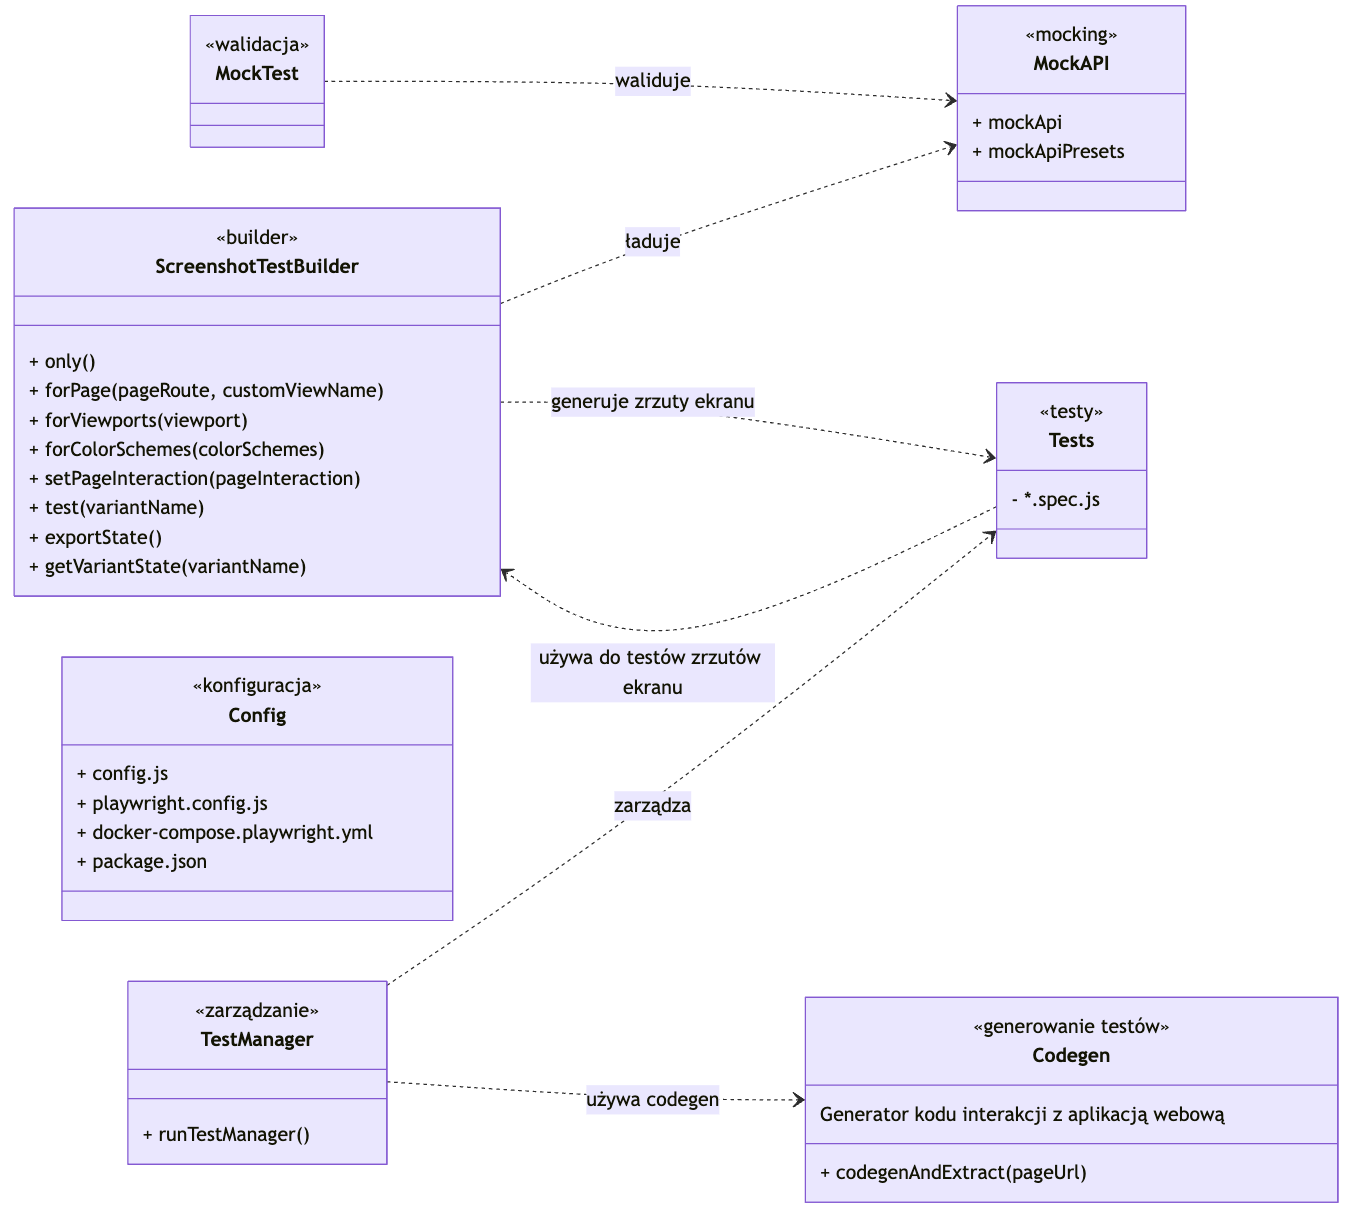
\includegraphics[width=0.95\textwidth]{diagram-projekt.png}
\caption{Diagram klas przedstawiający główne komponenty systemu}
\label{fig:diag-klas}
\end{figure}

Najważniejsze elementy widoczne na powyższym diagramie to:
\begin{itemize}
    \item \textbf{\texttt{ScreenshotTestBuilder}} -- centralny komponent służący do definiowania parametrów testów wizualnych (np. rodzaje widoków, warianty kolorów, interakcje na stronie). Udostępnia metody umożliwiające budowanie kompletnego scenariusza testowego.
    \item \textbf{\texttt{Tests}} (zawartość plików \texttt{*.spec.js}) -- zestaw testów wykorzystujących przygotowane warianty i funkcje \texttt{ScreenshotTestBuilder}. Każdy test może generować zrzuty ekranu w różnych konfiguracjach (urządzenie \emph{desktop}/\emph{mobile}, tryb \emph{light}/\emph{dark}, konkretna przeglądarka itp.).
    \item \textbf{\texttt{TestManager}} -- narzędzie CLI do uruchamiania testów, zarządzania nimi (np. edycja wariantów, usuwanie lub dodawanie interakcji) oraz współpracy z \texttt{codegen}.
    \item \textbf{\texttt{Codegen}} -- moduł pozwalający w półautomatyczny sposób wygenerować sekwencje interakcji z aplikacją (np. kliknięcia i wypełnianie formularzy), które następnie mogą być użyte w testach \texttt{spec.js}.
    \item \textbf{\texttt{Config}} -- pliki konfiguracyjne projektu (np. ustawienia rozdzielczości, ścieżki URL), dzięki którym w prosty sposób można dostosować testy do różnych środowisk.
    \item \textbf{\texttt{MockAPI}} i \textbf{\texttt{MockTest}} -- mechanizmy związane z symulowaniem wywołań API oraz walidacją, czy zdefiniowane dane \texttt{mock} są zgodne ze strukturą faktycznych odpowiedzi serwera.
\end{itemize}

\begin{figure}[H]
\centering
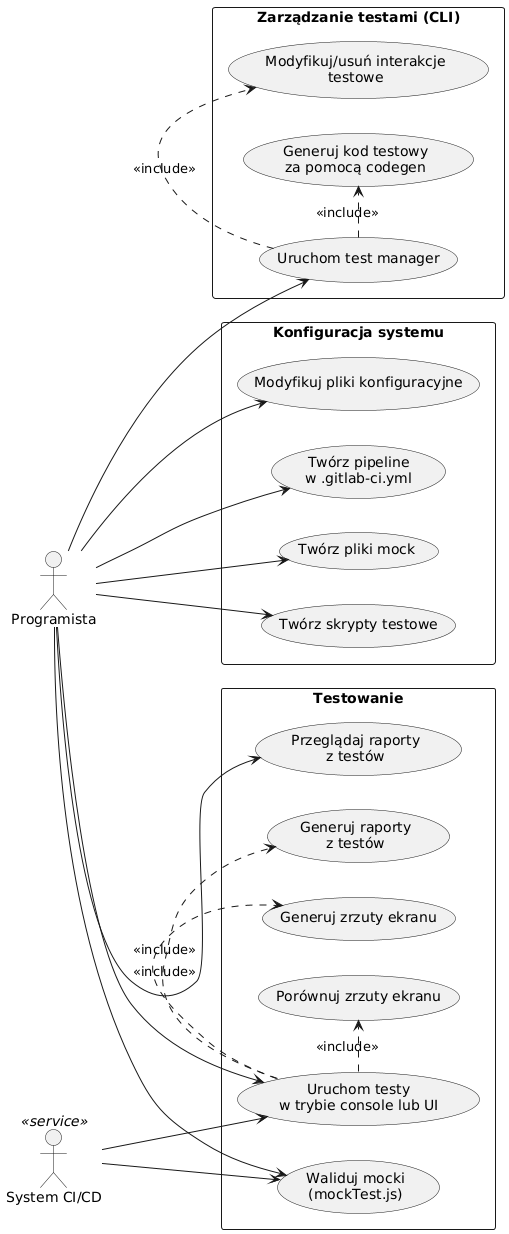
\includegraphics[width=0.7\textwidth]{use-uml.png}
\caption{Diagram przypadków użycia z perspektywy użytkownika i systemu CI/CD}
\label{fig:diag-use-case}
\end{figure}

Na diagramie przypadków użycia (rys.~\ref{fig:diag-use-case}) widoczna jest pełna interakcja pomiędzy:
\begin{itemize}
    \item \textbf{Programistą} -- tworzy i modyfikuje pliki konfiguracyjne, definiuje testy (\texttt{spec.js}) oraz może uruchamiać menedżer testów (\texttt{TestManager}).
    \item \textbf{Systemem CI/CD} -- automatycznie uruchamia testy (m.in. testy zrzutów ekranu i walidacje \texttt{mock}), generuje raporty i zarządza pipeline’em.
\end{itemize}
Zarówno człowiek (Programista), jak i \emph{System CI/CD} korzystają z tych samych głównych operacji: uruchamianie testów, weryfikacja \texttt{mock} i przeglądanie raportów. Ponadto Programista może w dowolnym momencie wywołać \texttt{TestManager}, by zmodyfikować scenariusze testowe (np. dodać nową interakcję na stronie).

\subsection{Zależność plików \texttt{spec.js} i \texttt{screenshotTestBuilder}}
\label{sec:zaleznosc-spec-builder}
Wszystkie pliki testowe oznaczone rozszerzeniem \texttt{.spec.js} w tym projekcie opierają się na funkcjonalnościach dostarczanych przez klasę \texttt{ScreenshotTestBuilder}. Oznacza to, że każdy test:
\begin{enumerate}
    \item Inicjalizuje \texttt{ScreenshotTestBuilder} (np. wywołując konstruktor i metody konfiguracyjne \texttt{forPage}, \texttt{setPageInteraction} itp.),
    \item Definiuje warianty testów (\texttt{test()} z nazwą wariantu bądź bez),
    \item Przechowuje i wykorzystuje stan zdefiniowany przez \texttt{ScreenshotTestBuilder}, aby ostatecznie wygenerować zrzuty ekranu w różnych kombinacjach ustawień.
\end{enumerate}

\noindent \textbf{Ścisła zależność} między \texttt{spec.js} a \texttt{screenshotTestBuilder} polega na tym, że:
\begin{itemize}
    \item \texttt{screenshotTestBuilder} udostępnia metody pozwalające na łatwe ustawienie dowolnych parametrów testu (np. \emph{viewport}, tryb kolorów, interakcje użytkownika),
    \item \texttt{*.spec.js} korzystają z tych metod w celu „zbudowania” gotowego scenariusza testowego,
    \item Każdy nowy plik \texttt{.spec.js} w praktyce \emph{musi} używać \texttt{ScreenshotTestBuilder}, dzięki czemu konfiguracja testów pozostaje spójna w całym projekcie.
\end{itemize}

\subsection{Rola \texttt{testManager} w zarządzaniu \texttt{spec.js} i codegenem}
\label{sec:rola-testManager}
\textbf{testManager} pełni w projekcie funkcję nadrzędnego narzędzia do zarządzania plikami \texttt{.spec.js} oraz wspiera Programistę w tworzeniu i modyfikowaniu interakcji testowych. Po uruchomieniu w trybie wiersza poleceń (CLI) pozwala m.in.:
\begin{itemize}
    \item \textbf{Przeglądać istniejące testy} -- użytkownik dostaje listę dostępnych plików \texttt{.spec.js} i może wybrać konkretny wariant testu do edycji.
    \item \textbf{Dodawać lub usuwać interakcje na stronie} -- \texttt{testManager} umożliwia szybkie wstawienie nowych kroków (np. kliknięcie przycisku, wypełnienie formularza) lub wyeliminowanie dotychczasowych akcji.
    \item \textbf{Korzystać z \textit{codegen}} -- integracja z \textit{Playwright codegen} umożliwia półautomatyczne generowanie scenariuszy testowych. Codegen nie jest częścią autorską tego projektu, lecz stanowi wbudowane narzędzie \textit{Playwright} do rejestrowania czynności w przeglądarce. Dzięki \texttt{testManager}, Programista może wywołać codegen, który „nagrywa” kroki wykonywane na stronie, po czym wygenerowany kod może zostać łatwo włączony do pliku \texttt{.spec.js}.
\end{itemize}

\noindent Głównym zadaniem \texttt{testManager} jest więc ułatwienie nawigacji w wielu plikach testowych i wsparcie w zarządzaniu różnymi wariantami testów (np. różne interakcje na tej samej stronie). Rozwiązuje to problem ręcznego dopisywania fragmentów kodu w \texttt{.spec.js}, bo dzięki integracji z codegen i mechanizmami CLI większość operacji można wykonać przy pomocy interaktywnych pytań i odpowiedzi.

\subsection{Działanie \texttt{mockApi} oraz \texttt{mockTest}}
\label{sec:dzialanie-mocki}
\textbf{\texttt{mockApi}} zapewnia w projekcie mechanizm definiowania sztucznych (testowych) odpowiedzi serwera. Dla wybranych endpointów API można zdefiniować, jakie dane mają być zwracane, dzięki czemu testy nie muszą opierać się na żywym środowisku produkcyjnym czy deweloperskim. Każda paczka \texttt{mock} (np. \texttt{/home/home.mock.js}) zawiera:
\begin{itemize}
    \item \textbf{Dane do zwrócenia} -- statyczne lub wygenerowane, opisujące np. przykładowy obiekt JSON, treść HTML czy obraz.
    \item \textbf{Parametry endpointu} -- wskazanie żądanej ścieżki (np. \texttt{/branding/}) lub zapytania (\texttt{?query=test}).
    \item \textbf{Presety} -- grupowanie kilku \texttt{mock} w zestawy, które można jednocześnie załadować w testach (np. \texttt{mockApiPresets.default}).
\end{itemize}

\noindent \textbf{\texttt{mockTest}} to z kolei moduł sprawdzający, czy zdefiniowane \texttt{mocki} są zgodne z prawdziwymi danymi, jakie zwraca produkcyjne API. Jego zadaniem jest:
\begin{itemize}
    \item \textbf{Pobranie realnej odpowiedzi} z wybranego endpointu w środowisku docelowym (np. \texttt{https://automationintesting.online/room/}).
    \item \textbf{Porównanie struktury} z danymi zadeklarowanymi w \texttt{mockApi}. Sprawdzana jest m.in. zgodność typu pól (np. czy \emph{roomPrice} to liczba), a dla obrazów weryfikowana jest zgodność formatu i rozmiaru.
    \item \textbf{Raportowanie ewentualnych różnic} -- w razie niezgodności \texttt{mockTest} informuje, który \texttt{mock} wymaga aktualizacji, by odzwierciedlać rzeczywisty stan API.
\end{itemize}

\noindent Dzięki temu \texttt{mockApi} nie „starzeje się” wraz ze zmianami w API, a deweloperzy mogą wciąż korzystać z lokalnych, izolowanych warunków testowych. Mechanizm \texttt{mockTest} pozwala zachować spójność danych testowych na przestrzeni rozwoju całej aplikacji.

\section{Szczegóły wybranych elementów (Rozdział 5.2)}
\label{sec:szczegoly-wybranych-elementow}
\textit{[Treść niezmieniona – pozostaje w projekcie tak, jak była]}

\subsection{API \texttt{screenshotTestBuilder} (metody \texttt{set}, \texttt{for} i inne) + przykład spec.js}
\label{sec:api-screenshotTestBuilder}
\textit{[Treść niezmieniona – pozostaje w projekcie tak, jak była]}

\subsection{Struktura plików \texttt{mock.js} (pola, za co odpowiadają) + przykład}
\label{sec:struktura-mockjs}
\textit{[Treść niezmieniona – pozostaje w projekcie tak, jak była]}

\subsection{Skrypty w \texttt{package.json}}
\label{sec:skrypty-package}
\textit{[Treść niezmieniona – pozostaje w projekcie tak, jak była]}

\subsection{\texttt{testManager}}
\label{sec:testManager}
\textit{[Treść niezmieniona – pozostaje w projekcie tak, jak była]}

\chapter{Kluczowe mechanizmy i biblioteki}

\section{Zasady organizacji projektu}
% - Kilka podrozdziałów, nie skupiamy się na kodzie, a na mechanizmach

\subsection{Struktura folderów i plików projektu; nazewnictwo zrzutów ekranu}
% - TU: opisać, jak zorganizowane są foldery \texttt{/tests}, \texttt{/mock} itp.
% - Wyjaśnić wzór nazwy screenshotu (np. \texttt{home-desktop-light-booking-chromium.png}) – skąd się bierze, co oznaczają segmenty

\subsection{Mechanizm tworzenia testów E2E przez \texttt{screenshotTestBuilder}}
% - TU: ogólnie, że builder generuje scenariusze testowe w oparciu o zadane parametry, a na końcu mamy \texttt{.spec.js} dla Playwright
% - Nie pokazywać kodu, jedynie proces

\subsection{Mechanizm \texttt{testManager} z wykorzystaniem \texttt{codegen}}
% - TU: wyjaśnić, że menedżer pozwala uruchomić codegen, przechwycić interakcje, wstawić je do \texttt{spec.js} itp.
% - Bez szczegółów implementacji, a tylko opis przepływu

\subsection{Mechanizm działania \texttt{mockTest}}
% - TU: przedstawić, że \texttt{mockTest} uruchamia walidację plików \texttt{.mock.js} z faktycznym API, porównuje odpowiedzi
% - Opisać koncepcję (schematy, porównania obrazów, weryfikacja JSON) bez wdawania się w kod


\section{Omówienie kluczowych bibliotek}
% - TU: lista najważniejszych bibliotek (np. \texttt{@playwright/test}, \texttt{inquirer}, \texttt{prettier}, \texttt{chalk}, \texttt{ajv} itp.)
% - Nie wchodzimy w szczegóły kodu, tylko opisujemy, do czego służą i jakie problemy rozwiązują

\section{Omówienie kluczowych miejsc w kodzie}
% - TU: wskazać, które pliki są najbardziej istotne dla działania (np. \texttt{testManager.js}, \texttt{screenshotTestBuilder.js}, \texttt{mockTest.js})
% - Krótko zaznaczyć, dlaczego są kluczowe (zarządzanie testami, generowanie screenshotów, weryfikacja mocków)
% - Nie opisywać szczegółów implementacyjnych, tylko ogólną rolę

\chapter{Przykłady użyć aplikacji}
{W tym rozdziale możesz zaprezentować, jak Twoje narzędzie działa w praktyce.}

\section{Uruchamianie narzędzia w trybie interaktywnym}
{Pokaż krok po kroku, jak użytkownik wypełnia formularz czy wybiera opcje w CLI, aby wygenerować testy. Zademonstruj końcowe pliki testowe.}

\section{Integracja z procesem CI/CD}
{Wyjaśnij, jak można włączyć wygenerowane testy do automatycznego pipeline’u, np. w GitLab CI, Jenkinsie, itp. Przedstaw przykładowy fragment konfiguracji.}

\chapter{Podsumowanie}
{Na koniec podsumuj swoją pracę, oceń jej efekty i zaproponuj kierunki rozwoju.}

\section{Wnioski końcowe}
{Opisz, w jakim stopniu udało się osiągnąć założone cele, co było największym wyzwaniem, co dało najwięcej satysfakcji/rezultatów.}

\section{Możliwości dalszego rozwoju}
{Opisz, jakie jeszcze funkcjonalności można by dodać do narzędzia, jakie usprawnienia byłyby przydatne, jakie biblioteki lub technologie mogłyby zostać wykorzystane w przyszłości.}

\begin{thebibliography}{9}
    \bibitem{roman2024} Roman, A., \& Zmitrow, K. (2024). \textit{Testowanie oprogramowania w praktyce: studium przypadków 2.0}.
    \bibitem{osherove2024} Osherove, R. (2024). \textit{Testy jednostkowe: świat niezawodnych aplikacji}.
    \bibitem{roman2024_case} Roman, A., \& Zmitrow, K. (2024). \textit{Testowanie oprogramowania w praktyce: studium przypadków}.
    \bibitem{roman2024_quality} Roman, A. (2024). \textit{Testowanie i jakość oprogramowania: modele, techniki, narzędzia}.
    \bibitem{circleci} CircleCI. (n.d.). What is End-to-End Testing? Pozyskano z \url{https://circleci.com/blog/what-is-end-to-end-testing/}
    \bibitem{playwright} Microsoft Playwright. (n.d.). Introduction to Playwright. Pozyskano z \url{https://playwright.dev/docs/intro}
\end{thebibliography}

\end{document}